%\usepackage{graphicx}%! suppress = EquationReference
\chapter{Аналитический раздел}

В данном разделе проводится анализ предметной области,
%анализ способов хранения данных в приложении и выбор оптимального, а также формализация требований к разрабатываемой программы.


\section{Анализ предметной области}

Время оборота самолета (\textit{англ.} TAT --- turnaround time) --- это общее время, которое требуется для выполнения всех необходимых операций между прилетом и отправлением самолета на следующий рейс.
Этот процесс включает в себя следующие этапы:
\begin{enumerate}[label=\arabic*)]
    \item обслуживание пассажиров и багажа;
    \item техническое обслуживание;
    \item управление нагрузкой;
    \item работы на стоянке.
\end{enumerate}

Вместе эти задачи определяют обслуживание самолета на земле и, следовательно, его TAT\@.
Этот параметр является ключевым показателем производительности любого воздушного судна.
Фактически, как авиакомпании, так и аэропортовые управляющие компании интересуются временем оборота: это один из наиболее важных договорных пунктов между двумя сторонами, поскольку он влияет на конкурентоспособность и прибыльность~\cite{trt-timeestimation}.

С момента посадки самолета на взлетно-посадочную полосу аэропорта до момента отправления на новый долгий полет остается мало времени для отдыха.
Обычно между рейсами есть всего несколько часов, и члены экипажа и технический персонал на земле должны разгрузить пассажиров и груз, очистить самолет и подготовить его к следующему рейсу.

Прежде чем самолет начнет спускаться в аэропорт, наземный экипаж уже готовится к его прибытию.
Стенд для стоянки самолета выделен аэропортом и освобожден от любых мусорных объектов, которые могут повредить самолет.
Кроме того, вся необходимая наземная техника припаркована вдали от области маневрирования самолета.
Как только стенд освобожден, включается управление стоянкой.
С помощью лазерных систем наведения пилоты могут управлять самолетом с повышенной точностью.

Как только самолет занимает правильное положение, система наведения начинает обратный отсчет до достижения точки остановки.
Затем необходимо установить стояночный тормоз, убедиться, что вспомогательная силовая установка (ВСУ) все еще работает, и закрыть все двери вручную перед остановкой двигателей.
Снаружи персонал на земле ожидает звука затухания двигателей и замедления вентилятора переднего двигателя.

Перед подходом к самолету землекоры будут искать маяк.
Маяк представляет собой мигающий красный свет сверху и снизу самолета, который, когда включен, сигнализирует землеобслуживающему персоналу, что безопасно подходить к самолету.
Как только маяк выключается, землекоры могут начинать выполнять свои обязанности, первая из которых включает установку ушей под колеса самолета.
Это позволяет гарантировать, что они не будут двигаться.

Когда двигатели остановлены, самолет использует ВСУ для питания.
Если ВСУ не работает, самолет должен быть подключен к наземному источнику питания перед остановкой двигателей.
Это может занять некоторое время, так как это требует подхода наземного персонала к самолету с подключением к наземному источнику питания, пока двигатели все еще работают.
В таких ситуациях землекоры должны быть осторожны и методично выполнять свои задачи для обеспечения безопасности.

После того как самолет надежно установлен и двигатели полностью остановлены, воздушный мост может быть перемещен к двери самолета, позволяя пассажирам покинуть самолет.
Обычно посадка/высадка пассажиров и заправка происходят с левой стороны, в то время как все остальные земные службы, такие как обслуживание питания и загрузка багажа и груза, выполняются с правой стороны.
Это позволяет выполнять различные сервисные работы одновременно.
Важно отметить, что багаж и груз разгружаются осторожно, чтобы обеспечить равновесие самолета.
В зависимости от нагрузки землекоры могут сначала разгрузить некоторые предметы из одного трюма, а затем приступить к другому, чтобы гарантировать, что самолет не упадет на хвост.

Что касается обслуживания туалетов, бак для отходов в задней части самолета опорожняется специалистом и техникой.
Последний пассажир выходит из самолета, и группа уборщиков и кулинаров сразу же заносит в кабину.
В соответствии с потребностями кабины пустые мусорные баки опорожняются, туалеты чистятся, мусор подбирается, собираются одеяла, меняются наволочки, и проводятся другие необходимые работы.
В то же время, кулинарные грузовики прибывают справа от самолета, чтобы загрузить продукты питания и напитки.

На данном этапе пилоты и члены экипажа проводят свой предварительный брифинг перед вылетом.
Маленький грузовик с питьевой водой подсоединяется к нижней части самолета сзади и накачивает воду в самолет.
Затем багаж и груз загружаются на самолет, что тщательно рассчитывается отделом планирования авиакомпании.
Перед взлетом инженеры внимательно осматривают самолет, проверяя уровни топлива и занимаясь мелкими деталями.

Примерно за час до вылета экипаж проверяет свое оборудование безопасности и аварийное снаряжение, а также подтверждает, что ничего не осталось от предыдущего рейса.
В галерах пересчитываются блюда и проверяются кулинарные запасы.
Как только все это сделано, пассажиры могут начать посадку на самолет.
В это время пилоты проводят проверки, загружают маршрут в компьютеры управления полетом, загружают прогнозируемые ветры и проводят брифинг перед вылетом.

Наконец, закрываются трюмные двери, пилоты запускают ВСУ для обеспечения самолета собственным электричеством, и заземленная электроэнергия отключается.
Тягач для отталкивания самолета располагается спереди от самолета, захватывает носовое колесо и позволяет самолету оттолкнуться от ворот.
Дверь для посадки пассажиров наконец закрывается, и авиамост убирается.
Теперь самолет готов к взлету~\cite{aircraft-trt}.


%\subsection{Анализ способов хранения данных в приложении}

%\subsubsection{БД и СУБД}
%
%База данных, сокращённо БД (\textit{англ.} DB --- database) --- совокупность структурированных взаимосвязанных данных, относящихся к определённой \linebreak предметной области и организованных таким образом, что эти данные могут быть использованы для решения многих задач многими пользователями~\cite{carpova}.
%
%Система управления базами данных, сокращённо СУБД (\textit{англ.} DBMS --- database management system) --- программная система, предназначенная для создания на ЭВМ общей базы данных для множества приложений, поддержания её в актуальном состоянии и обеспечения эффективного доступа пользователей к содержащимся в ней данным в рамках предоставленных им полномочий~\cite{carpova}.
%
%Основными функциями СУБД являются:
%\begin{enumerate}[label=\arabic*)]
%    \item управление данными во внешней памяти (обеспечение абстракции пользователя от организации данных);
%    \item управление данными во внутренней памяти (обеспечение работы с буферами оперативной памяти);
%    \item управление транзакциями (поддержка транзакций по принципу ``всё или ничего'', обеспечение их целостности);
%    \item журнализация (возможность восстановить состояние после сбоя);
%    \item поддержка языков БД (например, поддержка SQL).
%\end{enumerate}
%
%\subsubsection{Модели данных и способы классификации СУБД}
%
%Моделью данных  (\textit{англ.} data model) называют абстракцию, которая, будучи приложима к
%конкретным данным, позволяет пользователям и разработчикам трактовать их уже как информацию, то есть сведения, содержащие не только данные, но и взаимосвязь между ними.
%На рисунке~\ref{fig:data-models} приведена классификация моделей данных~\cite{carpova-t-s}.
%
%%\FloatBarrier
%\begin{figure}[h]
%    \begin{center}
%        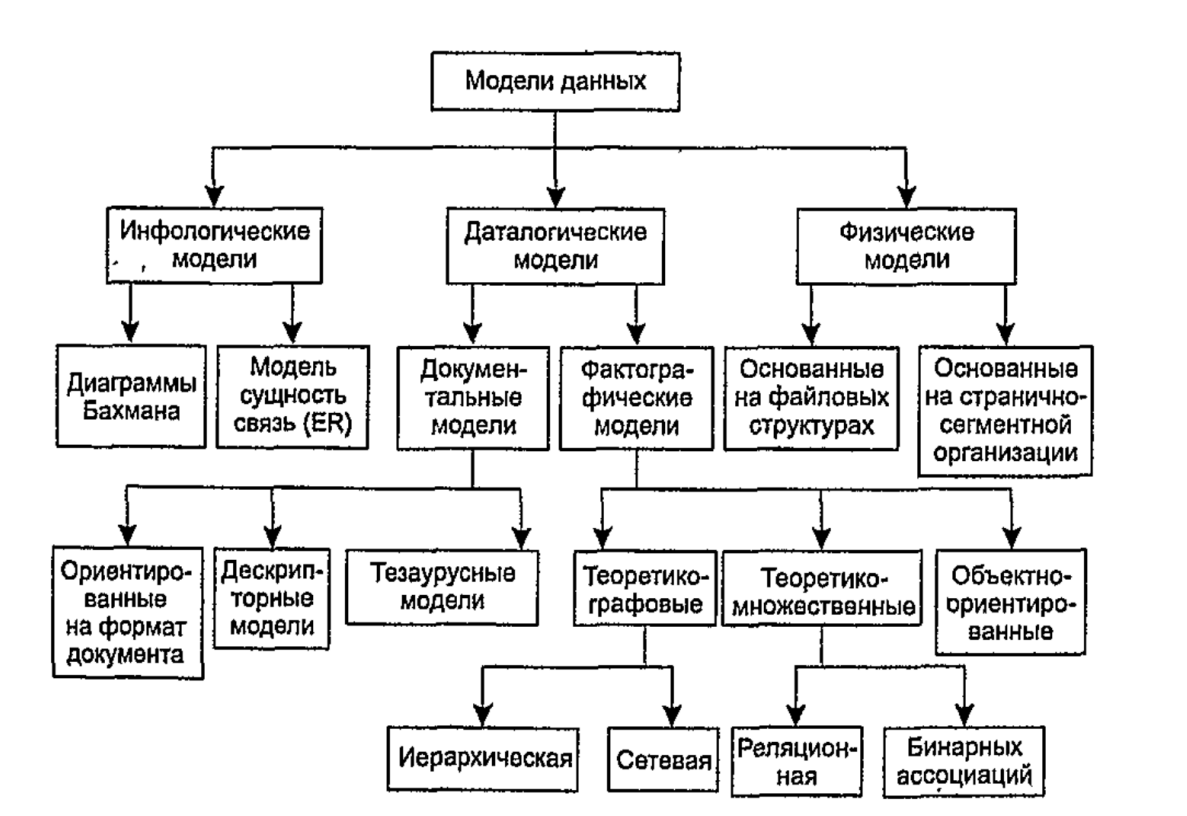
\includegraphics[scale=0.4]{inc/data-models}
%        \caption{Классификация моделей данных}
%        \label{fig:data-models}
%    \end{center}
%\end{figure}
%%\FloatBarrier
%
%\subsubsection{Модели хранения данных}
%
%По модели хранения данных выделяют следующие СУБД:
%
%\begin{enumerate}[label=\arabic*)]
%    \item дореляционные (инвертированые списки, иерархические и сетевые СУБД)
%    \item реляционные;
%    \item постреляционные.
%\end{enumerate}
%
%\subsubsection{Иерархическая модель данных}
%
%Иерархическая модель данных --- это одна из первых моделей баз данных, разработанная в 1960-х годах.
%Она представляет данные с использованием древовидных структур, где каждый узел содержит один родительский и несколько дочерних узлов.
%Эта модель хорошо подходит для отношений ``один ко многим'' (1:N), когда родительский объект связан с несколькими дочерними объектами.
%
%Иерархическая модель характеризуется простотой и легкостью реализации.
%Тем не менее, это накладывает некоторые ограничения при работе со сложными отношениями и избыточностью данных.
%Типичным представителем является Information Management System (IMS) фирмы IBM\@
%
%Ключевые особенности иерархической модели данных представлены ниже:
%\begin{enumerate}[label=\arabic*)]
%    \item древовидная структура;
%    \item один родительский узел может иметь несколько дочерних узлов, но дочерний узел может иметь только один родительский узел;
%    \item отношения родитель-потомок представлены через родительские указатели или вложенные наборы;
%    \item оптимизирован для перехода от родительского узла к дочернему, а не наоборот;
%    \item лучше всего подходит для отношений ``один ко многим''.
%\end{enumerate}
%
%Преимущества иерархической модели данных представлены ниже:
%\begin{enumerate}[label=\arabic*)]
%    \item просто и легко понять;
%    \item эффективен для поиска и хранения данных;
%    \item хорошо подходит для иерархических данных, таких как организационные диаграммы, файловые системы и таксономии;
%    \item целостность данных поддерживается посредством принудительных отношений родитель-потомок.
%\end{enumerate}
%
%Недостатки иерархической модели данных представлены ниже:
%\begin{enumerate}[label=\arabic*)]
%    \item ограниченная гибкость для обработки сложных отношений, таких как отношения ``многие-ко-многим'' (M:N);
%    \item потенциальная избыточность данных, поскольку дочерним узлам может потребоваться хранить повторяющуюся информацию о своем родительском узле;
%    \item не оптимизирован для доступа к данным посредством навигации между детьми и родителями или поиска неиерархических данных;
%    \item обновление или удаление данных может быть затруднено из-за жесткой иерархической структуры.
%\end{enumerate}
%
%
%
%\subsubsection{Сетевая модель данных}
%
%Сетевая модель данных была разработана в конце 1960-х годов как развитие иерархической модели.
%Онa расширяет иерархическую модель, позволяя узлу иметь несколько родительских и дочерних узлов.
%Эта гибкость позволяет сетевой модели данных представлять отношения ``многие ко многим'' (M:N), что делает ее подходящей для более сложных структур данных.
%К известным сетевым системам управления базами данных относится: DBMS, IDMS, TOTAL, VISTA\@.
%
%На рисунке~\ref{fig:network-models} представлена сетевая модель данных~\cite{carpova-t-s}.
%
%\begin{figure}[h]
%    \begin{center}
%        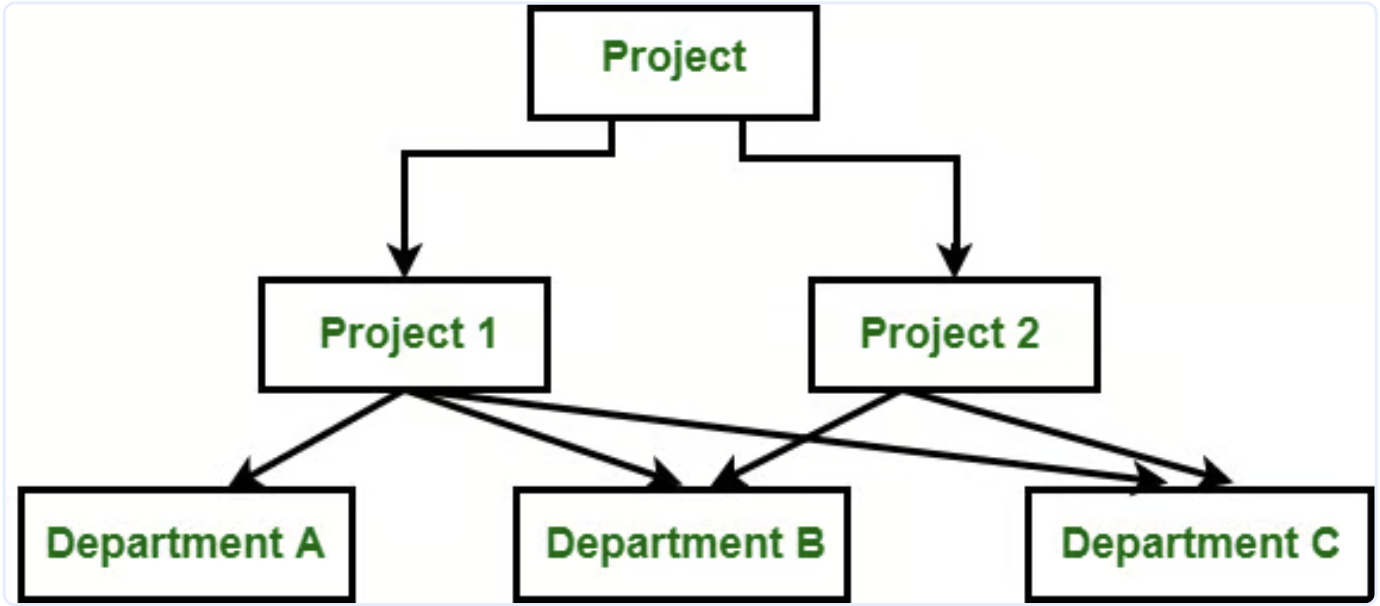
\includegraphics[scale=0.3]{inc/network-model}
%        \caption{Сетевая модель данных}
%        \label{fig:network-model}
%    \end{center}
%\end{figure}
%
%Расширение возможностей и гибкости моделирования достигается за счет сложности и производительности.
%Тем не менее, сетевая модель имеет свои преимущества и до сих пор используется в конкретных приложениях.
%
%Ключевые особенности сетевой модели данных представлены ниже:
%\begin{enumerate}[label=\arabic*)]
%    \item графоподобная структура;
%    \item каждый узел может иметь несколько родительских и дочерних узлов;
%    \item отношения представляются с помощью указателей записей, которые напрямую связывают связанные записи;
%    \item идеально подходит для отношений ``многие ко многим''.
%\end{enumerate}
%
%Преимущества сетевой модели данных представлены ниже:
%\begin{enumerate}[label=\arabic*)]
%    \item гибкость в представлении сложных отношений;
%    \item устраняет проблемы избыточности данных, обнаруженные в иерархической модели;
%    \item улучшена целостность данных за счет представления нескольких связей;
%    \item эффективен для поиска данных при прохождении связей.
%\end{enumerate}
%
%Недостатки сетевой модели данных представлены ниже:
%\begin{enumerate}[label=\arabic*)]
%    \item повышенная сложность по сравнению с иерархической моделью;
%    \item на производительность может повлиять сложность взаимоотношений;
%    \item обновление, удаление или вставка данных может оказаться более сложной задачей из-за взаимосвязанной структуры;
%    \item требует высокого уровня знаний для проектирования и обслуживания.
%\end{enumerate}
%
%
%
%\subsubsection{Реляционная модель данных}
%
%Реляционная модель данных была представлена доктором Эдгаром Коддом в 1970 году как способ упростить представление отношений данных.
%Реляционная модель представляет данные в виде отношений, которые по сути представляют собой таблицы со строками и столбцами.
%Каждая строка, также известная как кортеж, представляет одну запись данных, а каждый столбец соответствует атрибуту типа данных.
%
%Реляционная модель позволяет легко манипулировать данными и широко используется благодаря своей интуитивной природе, гибкости и поддержке языка структурированных запросов (\textit{англ.} SQL --- structured query language).
%Среди своих многочисленных преимуществ реляционная модель подчеркивает целостность данных и простоту запроса и изменения данных с помощью SQL\@.
%Примерами реляционных СУБД являются Oracle, Microsoft SQL Server, а также PostgreSQL\@.
%
%Ключевые особенности реляционной модели данных представлены ниже:
%\begin{enumerate}[label=\arabic*)]
%    \item данные представлены в виде таблиц со строками и столбцами;
%    \item строки представляют отдельные записи данных (кортежи), а столбцы представляют атрибуты типа данных;
%    \item первичные и внешние ключи представляют отношения.
%    \item данные обрабатываются с помощью SQL\@.
%\end{enumerate}
%
%Преимущества реляционной модели данных представлены ниже:
%\begin{enumerate}[label=\arabic*)]
%    \item простое и интуитивно понятное представление данных;
%    \item очень гибкий для представления различных типов отношений;
%    \item обеспечивает надежную целостность данных посредством ограничений первичного и внешнего ключа;
%    \item простое манипулирование данными и их получение с помощью SQL;
%    \item широко поддерживается различными системами управления базами данных (СУБД).
%\end{enumerate}
%
%Недостатки реляционной модели данных представлены ниже:
%\begin{enumerate}[label=\arabic*)]
%    \item может привести к проблемам с производительностью при работе с большими объемами данных или сложными запросами;
%    \item не оптимизирован для обработки иерархических или сетевых структур данных;
%    \item требует тщательного проектирования структур и связей таблиц, чтобы избежать избыточности данных и сохранить целостность данных.
%\end{enumerate}
%
%
%\subsubsection{Модель ``сущность-связь''}
%
%Модель ``сущность-связь'' (\textit{англ.} ER Model --- Entity--Relationship Model) --- это концептуальная модель данных, которая представляет данные в виде сущностей и их отношений.
%Основная цель модели ER --- обеспечить четкое, простое и графическое представление требований организации к данным путем определения ее компонентов, таких как сущности, атрибуты и связи.
%
%В модели ER сущность --- это реальный объект или концепция, которую хотим представить в базе данных, например человек, элемент или событие.
%Каждая сущность имеет набор атрибутов, описывающих ее характеристики или свойства.
%Например, в объекте ``клиент'' атрибуты могут включать имя, адрес, номер телефона и тд.
%
%Отношения в модели ER --- это ассоциация между двумя или более объектами.
%В модели ER существует три типа отношений: ``один-к-одному'', ``один-ко-многим'' и ``многие-ко-многим''.
%Очень важно правильно моделировать отношения, чтобы обеспечить целостность данных и эффективное использование базы данных.
%
%Диаграмма сущность--связь (\textit{англ.} ERD --- Entity--Relationship Diagram) — это популярный способ визуализации компонентов и их отношений в модели ER\@.
%ERD --- это графическое представление, в котором для обозначения сущностей, атрибутов и связей используются символы.
%Эта диаграмма помогает разработчикам баз данных быстро понять требования организации к данным и преобразовать их в подходящую физическую структуру базы данных~\cite{data-models}.
%
%
%
%\subsubsection{Архитектуры организации хранения данных}
%
%По архитектуре организации хранения и обработки данных и запросов выделяют следующие СУБД:
%
%\begin{enumerate}[label=\arabic*)]
%    \item файл-серверные --- базы данных хранятся на одном файл-сервере, а СУБД — на каждом устройстве, с которого отправляются запросы к БД.
%    Чтобы пользователь мог получить доступ к данным, у него на компьютере должна быть установлена и настроена СУБД.
%    Такие системы используют для локальных корпоративных сервисов: например, CRM, где хранятся данные о клиентах компании и документообороте.
%    Примеры: Microsoft Access, Paradox, dBase, FoxPro, Visual FoxPro;
%    \item клиент-серверные --- СУБД и базы данных размещены на одном сервере, к которому обращаются с запросами разные пользователи.
%    Получить доступ к данным через этот сервер можно с любого компьютера, специального ПО для этого не требуется.
%    Например, если это база данных интернет-магазина, где покупатели ищут разные товары.
%    Примеры: Firebird, MS SQL Server, Oracle, PostgreSQL;
%    \item встраиваемые --- локальные СУБД, которые встраиваются в приложение как отдельный модуль и используются для управления данными только внутри него.
%    Примеры: OpenEdge, SQLite, Microsoft SQL Server Compact~\cite{subd};
%    \item сервисно-ориентированные;
%    \item прочие (временные, пространственные, пространственно-временные).
%\end{enumerate}
%
%
%\subsubsection{Выбор типа СУБД}
%\subsubsection{PostgreSQL}
%
%Клиент--серверная реляционная СУБД, которая обладает значительной функциональностью и производительностью, при этом доступна бесплатно.
%Она также подходит для масштабных проектов с большими массивами данных и высокой нагрузкой.
%
%В качестве основного языка запросов используется SQL, но СУБД также поддерживает его расширения на базе языков программирования: PL/Perl, PL/Python и PL/Java.
%Одно из главных преимуществ PostgreSQL в том, что здесь нет ограничений по размеру баз данных и числу записей в таблицах.
%
%\subsubsection{MySQL}
%
%Реляционная СУБД клиент--серверного типа, которая подходит для средних и небольших команд или проектов.
%Программа для работы с базами данных обладает простым и удобным интерфейсом и доступна для свободного пользования, поддерживает множество разных форматов таблиц и постоянно расширяет свои возможности.
%
%СУБД работает онлайн с высокой скоростью и позволяет хранить до 50 млн единиц данных.
%Однако её функциональность всё же хуже, чем у PostgreSQL. MySQL используют для хранения и управления данными сайтов и интернет-магазинов, среди которых Facebook, Twitter, Alibaba, Wikipedia.
%Она также может работать в комбинации с другими популярными СУБД.
%
%\subsubsection{Microsoft SQL Server}
%
%Реляционная СУБД, расширенную платную версию которой используют в крупных компаниях.
%Бесплатная версия Express подходит для небольших проектов с объёмом данных до 10 Гб.
%
%Система позволяет автоматизировать рутинные задачи: например, изменить размер файла или управлять памятью.
%Здесь удобно хранить данные со сложной структурой и быстро находить нужное за счёт простого поиска.
%
%В систему можно выгружать данные из других программ Microsoft (например, Access и Excel), а также вносить изменения в режиме онлайн.
%Для запросов в СУБД используется расширение SQL T--SQL (Transact--SQL).
%
%\subsubsection{MongoDB}
%Документная система управления NoSQL, где данные хранятся в виде JSON-файлов (\textit{англ.} JavaScript Object Notation), то есть текстовых документов в формате, основанном на JavaScript.
%Его же СУБД поддерживает в качестве языка запросов вместо SQL\@.
%
%Вместо таблиц, как это принято в реляционных СУБД, в MongoDB данные хранятся в виде коллекций, то есть групп документов.
%Это бесплатная программа для работы с БД с открытым кодом, которая позволяет хранить любые данные, если их перевести в формат JSON. Такие свойства делают её практически универсальной и легко масштабируемой.
%
%Эта СУБД подходит для работы с большими данными разных типов и из множества разных источников.
%Данные автоматически распределяются между разными базами так, чтобы оптимизировать нагрузку и ускорить обработку запросов.
%MongoDB используют для хранения локальных данных такие компании, как Google, Facebook, Twitter, IBM, Forbes, а также многие интернет--магазины.
%
%
%\subsubsection{SQLite}
%
%Компактная СУБД, которая подходит для небольших проектов.
%Она состоит из одного файла и встраивается в IT--инфраструктуру в виде библиотеки, не задействуя серверы и специальные службы.
%Все базы данных хранятся на одном устройстве.
%
%SQLite подходит для небольших сайтов и приложений с ограниченным трафиком и объёмом данных, а также сервисов, где нужно прочитать или сохранить файлы на диск.
%СУБД работает на компьютерах, смартфонах, ТВ, приставках и беспилотниках, не требует администрирования и поддержки.
%В качестве языка запросов здесь используется С.


\section{Анализ существующих решений}
\section{Формулировка требований к разрабатываемой базе данных}
\section{Формализация информации, хранимой в базе данных}
\section{Система ролей}
\section{Выбор модели базы данных}

**TO DO**
%\subsection{Группы пользователей}
%
%Выделим группы пользователей разрабатываемой системы, исходя из \linebreak предметной области поставленной задачи.
%
%Выделяется 4 типа пользователей: системный администратор, главный врач, врач и работник регистратуры.
%Предусмотрим набор возможностей для каждого типа пользователей.
%
%Набор возможностей системного администратора:
%\begin{itemize}[leftmargin=1.6\parindent]
%    \item[---] вход в систему;
%    \item[---] регистрация новых пользователей;
%    \item[---] настройка уровней доступа.
%\end{itemize}
%
%Набор возможностей главного врача:
%\begin{itemize}[leftmargin=1.6\parindent]
%    \item[---] вход в систему;
%    \item[---] учёт пациента;
%    \item[---] учёт сотрудника;
%    \item[---] просмотр расписания врачей и кабинетов.
%\end{itemize}
%
%Набор возможностей врача:
%\begin{itemize}[leftmargin=1.6\parindent]
%    \item[---] вход в систему;
%    \item[---] приём пациента;
%    \item[---] управление электронной медицинской картой пациента;
%    \item[---] просмотр расписания врачей и кабинетов.
%\end{itemize}
%
%Набор возможностей работника регистратуры:
%\begin{itemize}[leftmargin=1.6\parindent]
%    \item[---] вход в систему;
%    \item[---] регистрация нового пациента;
%    \item[---] учёт пациента;
%    \item[---] просмотр расписания врачей и кабинетов.
%\end{itemize}
%
%Данные наборы возможностей сотрудников поликлиники можно объединить в диаграмму, приведённую на рисунке~\ref{fig:usecase}.
%
%\begin{figure}[h!]
%    \centering
%    \captionsetup{justification=centering}
%    \includegraphics[width=150mm]{usecase.png}
%    \caption{Диаграмма вариантов использования для поставленной предметной области}
%    \label{fig:usecase}
%\end{figure}
%
%
%
%\subsection{Категории данных}
%
%Основываясь на анализе предметной области, можно выделить следующие категории данных:
%\begin{itemize}[leftmargin=1.6\parindent]
%    \item[---] пользователь системы;
%    \item[---] пациент поликлиники;
%    \item[---] сотрудник поликлиники;
%    \item[---] должность в поликлинике;
%    \item[---] приём пациента;
%    \item[---] расписание;
%    \item[---] медицинская карта пациента;
%    \item[---] состояние пациента;
%    \item[---] договор с пациентом;
%    \item[---] паспорт;
%    \item[---] адрес.
%\end{itemize}
%
%Информация, соответствующая каждой категории, содержится в таблице~\ref{table:category-info}.
%
%\clearpage
%
%\begin{table}[H]
%    \begin{center}
%        \captionsetup{justification=raggedright,singlelinecheck=off,margin=5mm}
%        \caption{Информация для выделенных категорий данных}
%        \begin{tabular}{| c | c |}
%            \hline
%            Категория данных & Информация \\
%            \hline
%            Пользователь системы & логин, пароль, сотрудник, уровень доступа \\
%            \hline
%            Пациент поликлиники & \makecell{паспорт, адрес, телефон,\\ домашний телефон, почта}  \\
%            \hline
%            Сотрудник поликлиники & \makecell{паспорт, должность, \\дата наёма, дата увольнения} \\
%            \hline
%            Должность в поликлиники & название должности, зарплата \\
%            \hline
%            Приём пациента &
%            \makecell{врач, пациент, дата, \\
%            динамика состояния, назначение,\\
%            примечание, состояние}\\
%            \hline
%            Расписание &\makecell{сотрудник, день недели, кабинет, \\
%            время начала работы, время \\окончания работы}\\
%            \hline
%            Медицинская карта пациента & паспорт, договор, дата постановки на учёт \\
%            \hline
%            Состояние пациента & \makecell{общее состояние, рост,\\ вес, пульс, давление, \\температура, прочее }\\
%            \hline
%            Договор с пациентом & \makecell{номер договора, пациент, \\дата заключения, дата \\окончания, дата обновления} \\
%            \hline
%            Паспорт & \makecell{фамилия, имя, отчество, \\
%            дата рождения, пол, серия, \\
%            номер, дата выдачи, место выдачи} \\
%            \hline
%            Адрес & страна, город, улица, дом, этаж, квартира \\
%            \hline
%        \end{tabular}
%        \label{table:category-info}
%    \end{center}
%\end{table}
%
%\subsection{Формализация задачи}
%
%При помощи диаграммы сущность-связь (\textit{англ.} entity-relation diagram) можно выделить ключевые сущности, их атрибуты, а также типы и род связей между этими сущностями.
%На основе даанных связей позже будет построоена диаграмма базы данных, поскольку связи между сущностями поозволяют точнее определить связи между объектами базы данных.
%Диаграмма сущность-связь для поставленной предметной области приведена на рисунке~\ref{fig:er}.
%
%\begin{figure}[h!]
%    \centering
%    \captionsetup{justification=centering}
%    \includegraphics[angle=90, width=150mm]{er.png}
%    \caption{Диаграмма сущность-связь для поставленной предметной области}
%    \label{fig:er}
%\end{figure}
%
%
%%
%\subsection*{Вывод}
%В данном разделе был проведён анализ предметной области (информационные системы для частных поликлиник), а также проведён анализ существующих СУБД.
%Как СУБД, при помощи которой будет решаться поставленная задача, была выбрана реляционная клиент-серверная СУБД.
%Были приведены диаграммы сценариев использования информационной системы, проанализированы категории даных, приведена диаграмма сущность-связь, поясняющая суть связей между выделенными сущностями, соответствующими категориям данных.

